\documentclass[12pt]{article}
\usepackage[utf8]{inputenc}
\usepackage{amsmath}
\usepackage{graphicx}
\usepackage{caption}
\usepackage{subcaption}
\usepackage{url}
\usepackage{setspace}
\title{Dissertation Proposal}
\author{Curran Kelleher}
\date{3/13/2014}
\begin{document}
\maketitle 

\begin{onehalfspacing}
\begin{abstract}
There is immense potential value in public data that is not being realized. While publicly available data sets are published on the Web, it is difficult to realize their full value in practice because they are made available using numerous different formats and protocols. The heterogeneity of formats and protocols used makes it difficult to combine and analyze data sets together, and hinders the development of analysis and visualization tools. In this proposal, we present preliminary designs for novel data structures and algorithms supporting integration and interactive visualization of data sets from multiple sources, based on the data cube concept. The proposed data representation framework will allow many data sets from different sources to be combined together and visualized using interactive visualization dashboards with multiple linked views. The focus will be on publicly available data, however the proposed framework can be applied to any data collection whose components can be conceptually modeled as data cubes.
\end{abstract}
\end{onehalfspacing}

\pagebreak

\tableofcontents

\pagebreak

\begin{doublespace}
\section{Introduction}
Consider the data from the US Census that covers population statistics for US States from 1950 to 2010. Consider also population statistics from the United Nations covering World Countries from 1970 to 2012. These two data sets may use different identifiers for years and geographic regions, but they cover an overlapping conceptual data space of time, geography and population. From these two data sets it is possible to create a visualization dashboard with a map of the world showing population as color and a corresponding line graph showing population for each region as lines. If the user views the whole world, the UN population data is shown for each country. If the user zooms into the US, US Census data is shown for each state. If the user selects a point of time in the line graph, the data shown on the map is from that point in time. If the user pans and zooms on the map, the lines in the line graph update to only show the regions visible on the map.

The contributions of this dissertation are novel data structures and algorithms for integration and interactive visualization of many data sets from multiple sources, based on the data cube concept. The focus will be on public data, however the techniques can be applied to any data collection. The proposed data representation framework will allow data sets to be combined together and visualized using interactive visualization dashboards like the one described, giving users the sense that the data exists within a single unified structure. The framework is designed to be able to represent and integrate an arbitrary number of data sets created independently of one another, and expose the integrated structure to reusable visualization tools that can be combined together in dashboard layouts with multiple linked views. The proposed data representation and visualization framework is fundamentally new, and will allow heterogeneous data sets to be explored in a unified way that was never before possible. 

Data cubes, also known as OLAP (OnLine Analytical Processing) cubes, can represent data that contains measures aggregated (typically using sum or average) along categorical hierarchies. The data cube concept emerged from the field of data warehousing as a way to summarize transactional data, allowing analysts to get a bird's eye view of company activities. The term OLAP stands in contrast to OLTP (OnLine Transaction Processing), which is the part of the data warehouse system that ingests and stores data at the level of individual transactions or events. After the ETL (Extract, Transform and Load) phase of the data warehouse flow, the data is analyzed by computing a data cube from the transactional data.

The data cube concept and structure can be used to model existing data as well. Publicly available data sets (often termed ``statistical data'') may be considered as pre-computed data cubes if they contain aggregated measures (also called ``indicators'', ``metrics'' or ``statistics'') across time, geographic space, and other dimensions such as gender, age range, ethnicity or industry sector. With this approach, it is possible to model many data sets together using shared dimensions and measures which will allow integration of many data sets together in a single structure. Existing OLAP technologies assume that the data cubes will be computed from a relational source, and are not designed to handle integration of pre-computed data cubes that may use inconsistent identifiers for common dimensions and measures. Therefore the application of the data cube concept to integration and visualization of many pre-computed data cubes, while theoretically plausible, requires the development of novel data structures and algorithms that extend the data cube model to handle integration of pre-computed data cubes that may use inconsistent identifiers for common dimensions and measures.

The envisioned data representation and visualization framework can serve as a digital telescope into the universe of phenomena on Earth via publicly available data. For example, consider public data sources such as the United Nations, the US Census, the US Bureau of Labor Statistics, or the US Centers for Disease Control. These organizations and hundreds of others around the world provide publicly available data about various topics including population statistics, public health, distribution of wealth, quality of life, economics, the environment, and many others. By unifying these data sources and providing users with tools to explore them visually, a deeper understanding of the world can be gleaned by anyone through the lens of public data.

There is immense potential value in public data that is not being realized. The ability to visually explore public data lends itself to applications in education, journalism, and public policy. Especially in the era of ``Big Data'', it is increasingly valuable for organizations and individuals to have the ability to analyze large quantities of data from various sources that varies across time, space, and other dimensions. In addition, publicly available data can provide context for business-centric proprietary data analysis activities.

\begin{figure}[h!]
  \centering
  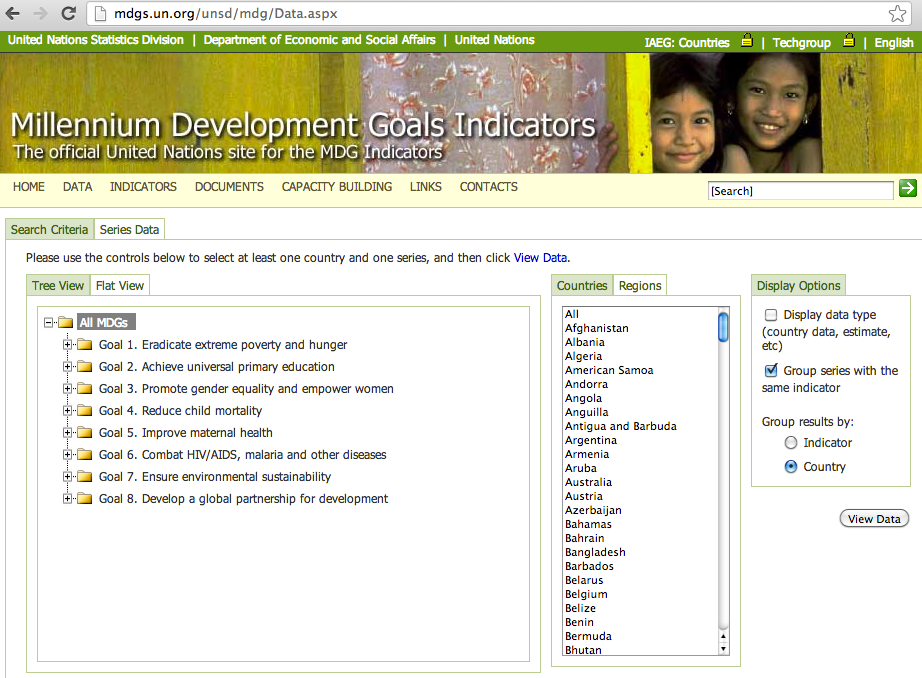
\includegraphics[width=\textwidth]{figures/MDGInterface.png}
  \caption[Millenium Development Goals Web Interface.]
   {The Web-based interface provided for navigating the United Nations Millenium Development Goals Indicator data sets \cite{mdgDataUI}. This is one example of the variety of formats and protocols used for making public data available on the Web.}
  \label{fig:MDGInterface}
\end{figure}

\begin{figure}[h!]
  \centering
  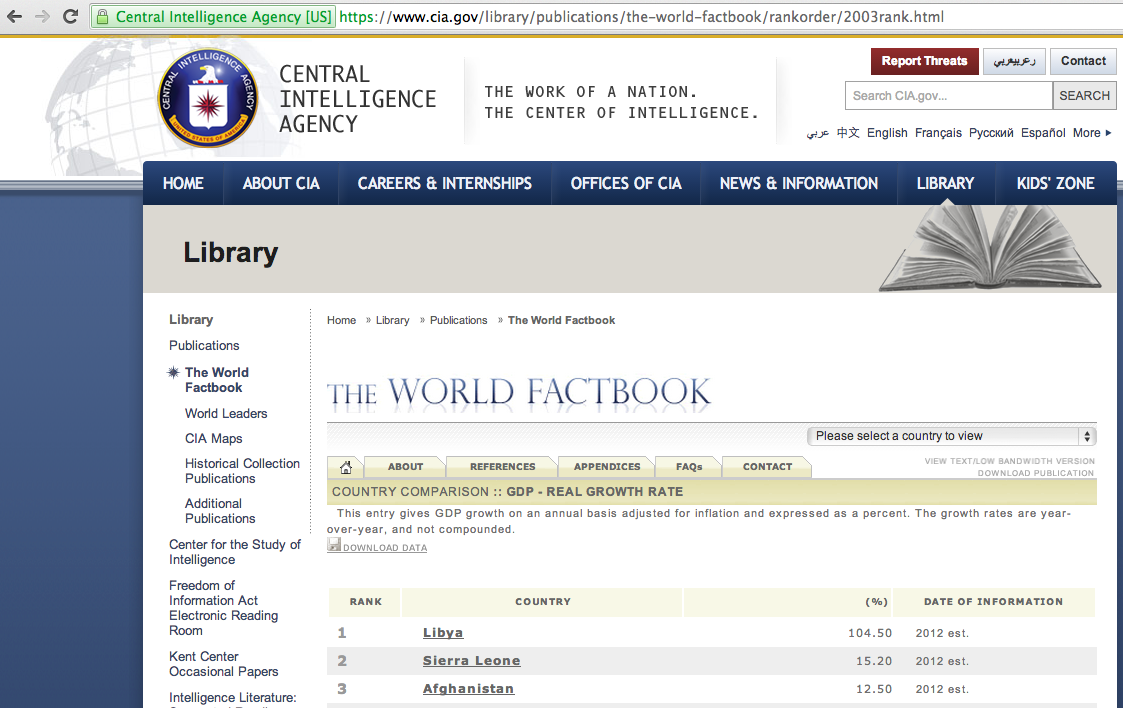
\includegraphics[width=\textwidth]{figures/CIAWorldFactbook.png}
  \caption[CIA World Factbook Web Interface.]
    {The Web-based interface for downloading data from the CIA World Factbook \cite{ciaWorldFactbookData}. A data download link is provided that yields a text file using a nonstandard table format. This is a second example of the variety of formats and protocols used for making public data available on the Web.}
  \label{fig:ciaWorldFactbook}
\end{figure}

\begin{figure}[h!]
  \centering
  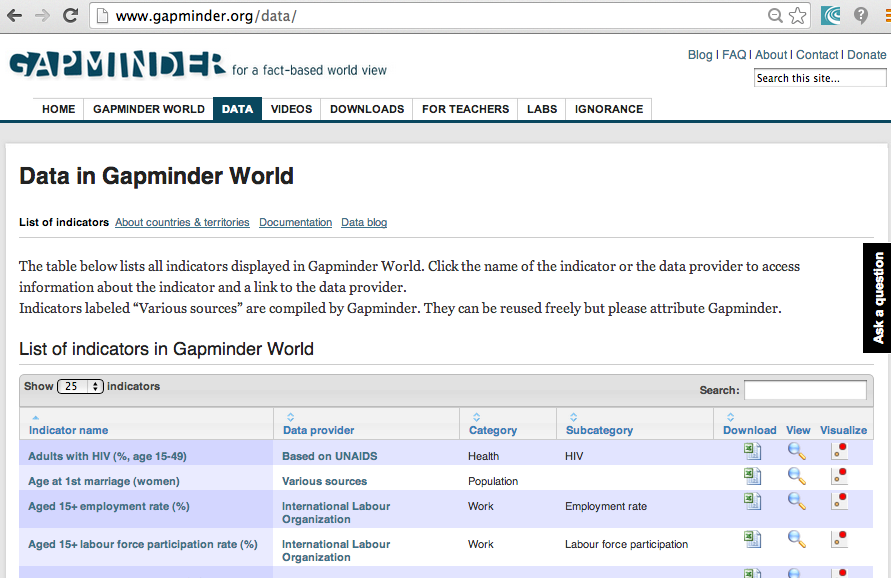
\includegraphics[width=\textwidth]{figures/gapminderData.png}
  \caption[GapMinder Data Access User Interface.]
    {The Web-based interface for downloading data harvested by the GapMinder project \cite{gapminderData}. A data download link is provided for each indicator that yields an Excel spreadsheet hosted using Google Docs.}
  \label{fig:gapminderData}
\end{figure}

\begin{figure}[h!]
  \centering
  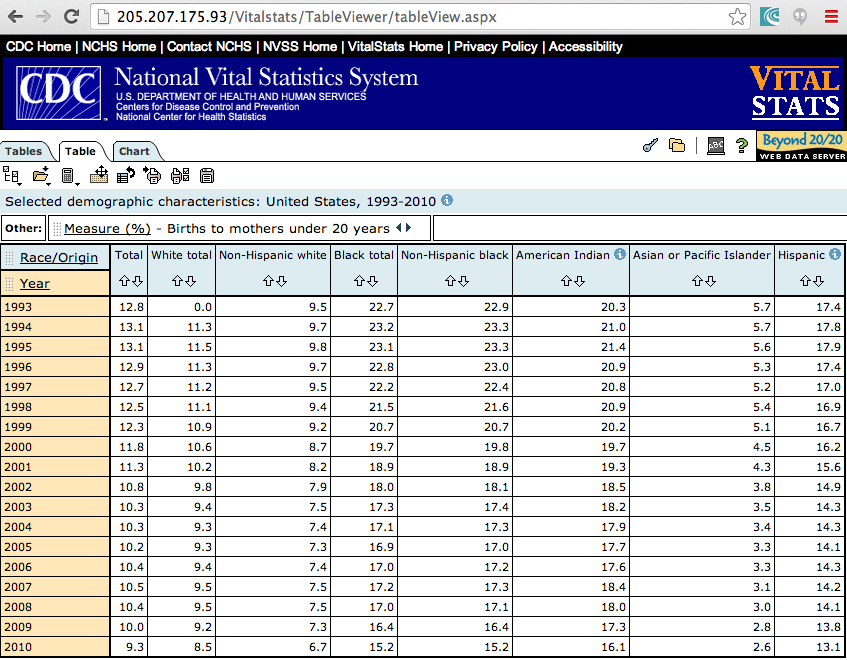
\includegraphics[width=\textwidth]{figures/CDCVitalStatsUI.png}
  \caption[CDC Vital Statistics.]
    {The Web-based pivot table user interface for downloading data from the US Centers for Disease Control about births to mothers under age 20 by demographic and year \cite{CDCVitalStatsUI}. The product powering this interface is the Beyond 20/20 Web Data Server \cite{beyond2020webDataServer}. In this interface a ``download'' button is provided that yields data in CSV (Comma Separated Value) format.}
  \label{fig:CDCVitalStatsUI}
\end{figure}

\begin{figure}[h!]
  \centering
  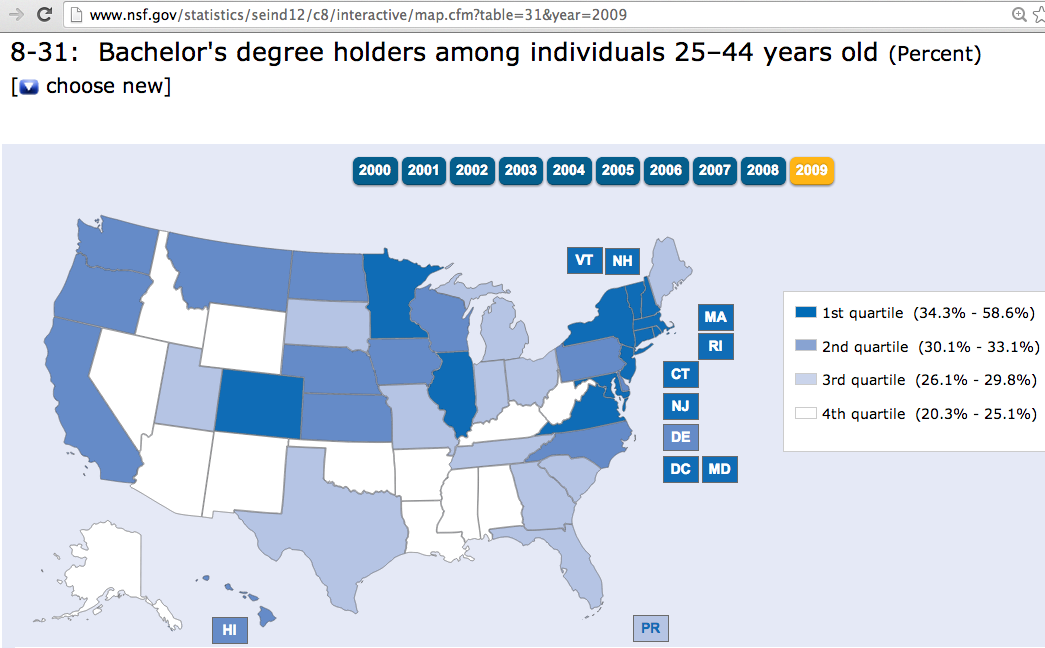
\includegraphics[width=\textwidth]{figures/nsfBachelorsDegrees.png}
  \caption[NSF Bachelors Degrees Statistics.]
    {An interactive visualization of bachelors degree statistics provided by the National Science Foundation site \cite{nsfBachelorsDegrees}. This is an example of an extremely limited visualization tool provided along with a public data set.}
  \label{fig:nsfBachelorsDegrees}
\end{figure}

While publicly available data sets are available on the Web, it is difficult to realize their full value in practice. The difficulty stems from the fact that they are made available using numerous different representations and protocols. For example, some data sets are made available as CSV files, Excel spreadsheets (such as the one shown in figure \ref{fig:unPopExcel}), or must be navigated using a Web-based user interface such as the ones shown in figures \ref{fig:MDGInterface}, \ref{fig:ciaWorldFactbook}, \ref{fig:gapminderData} and \ref{fig:CDCVitalStatsUI}. Sometimes visualization interfaces are provided for public data, such as in figure \ref{fig:nsfBachelorsDegrees}, however these tools are typically extremely limited in scope and hard-coded to the data set at hand. The heterogeneity of formats and protocols used makes it difficult to combine and analyze data sets together, and hinders the development of analysis and visualization tools. With the tools available today such as D3.js, creation of Web-based interactive data visualizations involves hard coding one-off projects to a particular data set.

Ideally, anyone should be able to apply interactive visualization techniques to public data easily. This dissertation focuses on the challenges in making this a reality, and offers a solution based on the data cube concept. The proposed framework will reduce the effort required to create Web-based data visualizations by linking reusable visualization templates with public data sets that have been imported into our generalized data representation framework.

Many, but not all, data sets can be modeled as data cubes. Since data cubes are only capable of representing data that has been aggregated along categorical dimensions, there are many classes of data that do not fit within the model. For example, a database containing the details of transactions in a supermarket would not be appropriate to model as a data cube. Each entry of a customer purchase may contain a listing of items purchased, how it was paid for, and the date and time the purchase was made. This kind of data fits well into the relational model, but is not appropriate to model as a data cube. Data cubes represent only aggregated summaries, not individual events. In the case of grocery store database containing the transactions for many grocery stores in different regions, while the individual transaction entries cannot be modeled as a data cube directly, a data cube can be constructed from the transactional data by aggregating measures such as ``amount paid'' and ``number of items purchased'' along dimensions such as ``time'', ``region'' and ``product category''. This is a typical data warehouse scenario, where a business aggregates transactional data into a data cube in order to analyze company activities in a summary view.

The key characteristics that allow a given data set to be modeled as a data cube are as follows:

\begin{itemize}
\item The data set contains numeric fields (termed ``measures'') that represent aggregated summaries using sum, average, or some other aggregation operator.
\item The measures of the data set are aggregated along one or more sets of discrete categories or entities (termed ``dimensions''). These dimensions can be either unordered, ordered, or hierarchical.
\end{itemize}

Data sets that have the following qualities may not be modeled as a data cube (although it may be possible to compute data cubes that summarize data sets like these):

\begin{itemize}
\item The data set represents a graph. Graph data such as social network connections or links between Web pages is not supported by the data cube model.
\item The data set contains relational data with a one-to-many relation. For example, a database of transactions in a grocery store where one transaction has many items. Items containing lists of other items cannot be represented using the data cube model. However, one may consider transforming data sets like this such that the nested lists are summarized by some measures (such as total cost or number of items) so the data cube model can be applied.
\item The data set contains entries for individual discrete events or transactions. Data sets with this quality cannot be modeled directly as data cubes, however it may be possible to compute data cubes by aggregating them using OLAP techniques from data warehousing.
\end{itemize}

Public data tends to be particularly well suited to the data cube model because it typically contains measures about people (or byproducts of human activities) distributed across time, space (geographic regions) and other dimensions such as gender or age range. For example, the public data available in the Gapminder visualization tool contains measures (such as ``number of adults with HIV/AIDS'' and ``child mortality'') aggregated across countries and years \cite{gapminderData}. This partitioning of space into countries and time into years is one choice of levels in the space and time hierarchies, but the data cube model is more general in that it can support multiple levels of detail in both the Space dimension (e.g. Continents, Countries, States, Counties, and Metropolitan Areas) and the Time dimension (e.g. millenia, centuries, years, months, days, hours and minutes). Therefore any public data sets that contain measures (also called statistics, indicators or metrics) aggregated along any resolution of time and space can be modeled as data cubes.

When multiple data sets are modeled as data cubes, they can be integrated into a single structure. Based on the common dimensions and measures shared between data sets, an integrated heterogeneous data cube structure can be created from an arbitrary number of data sets from multiple sources. Interactive visualization techniques can be applied to this integrated structure, yielding fundamentally new ways of exploring and presenting multiple data sets.

\pagebreak
\section{Expected Contributions}
The expected contributions of this dissertation include the following:
\begin{itemize}
\item Novel data structures and algorithms for data cube integration. Existing formats, protocols and models only consider the case of homogeneous data cubes computed from a single source of relational data, and do not handle the case of integrating many pre-computed data cubes from multiple sources. Data integration has been well studied for relational data, but data integration methods have not been applied to OLAP cubes, which present unique challenges including management of dimension hierarchies and measures that are ``universal'', or shared by many data sources.
\item A conceptual framework that links the integrated data cube structure with existing data visualization theory and techniques. Much work has been done concerning ``Visual OLAP'' \cite{mansmann2008visual}, however the visualization approaches for OLAP cubes have not been extended to handle the rich heterogeneous structure introduced by integrating many data cubes from multiple sources.
\item A framework for defining visualization dashboards with multiple linked views for interactively exploring integrated data cubes. Interactions between multiple views for OLAP cubes have been considered, but our proposed integrated data cube structure affords a richer set of interactions that goes beyond traditional OLAP operations such as drill-down, roll-up, slice and dice.
\end{itemize}

These contributions will advance the field of computing and data visualization by enabling the development of tools for integrating and visualizing heterogeneous data sets in ways never before possible.
\pagebreak
\section{Related Work}
\subsection{Data Representation}
In today's world of ``information overload'', data takes many forms. Perhaps the most familiar data representation system today is Microsoft Excel, which is capable of representing data tables as well as complex operations across the data values \cite{eick2000visualizing}. Many organizations use Excel to manage data or make data available as Excel spreadsheets. For example, the United Nations Department of Economic and Social Affairs makes their population statistics available in Excel format (see figure \ref{fig:unPopExcel}).

\begin{figure}[h!]
  \centering
  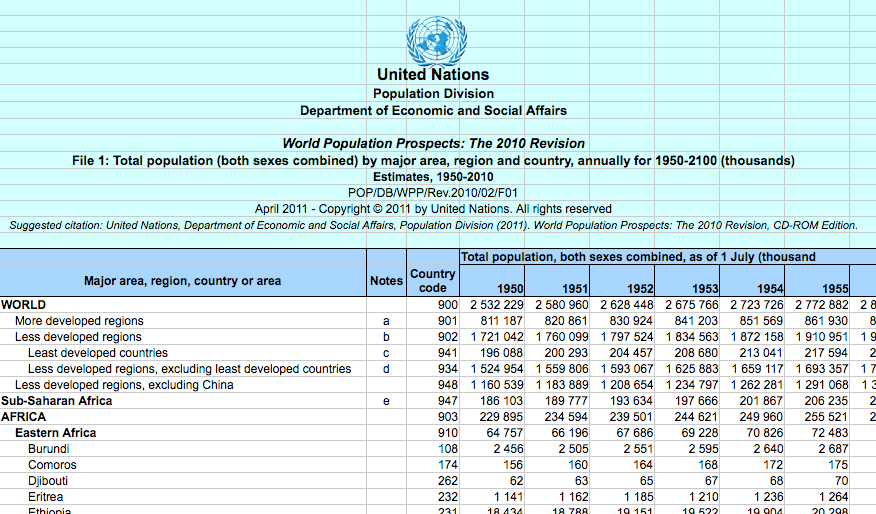
\includegraphics[width=\textwidth]{figures/UN_World_Population_Spreadsheet.png}
  \caption[United Nations population estimates spreadsheet.]
   {The United Nations Population Prospects data set \cite{unPopData}, made available in Excel format. This is another example of a public data set that could be imported into our data representation framework.}
  \label{fig:unPopExcel}
\end{figure}

Relational database systems provide a mature data management solution and are widely adopted \cite{ramakrishnan2000database}. The relational model has well understood theoretical underpinnings such as the relational algebra \cite{clifford1985algebra}. Data warehouse systems are typically built on the relational model, and augmented by multi-scale aggregated data structures called data cubes, also known as OLAP (OnLine Analytical Processing) cubes \cite{gray1997data} \cite{codd1993providing}. Data cubes contain summaries of the collection of facts stored in a relational database \cite{chaudhuri1997overview}. For example, a data cube may contain how much profit was made from month to month subdivided by product category, while the relational database may contain the information associated with each individual transaction. Because data cubes provide a higher level of abstraction, they are a widely used method of data abstraction for supporting visualization and analysis tasks. Kimball pioneered the area of ``Dimensional Modeling'', which concerns constructing data warehouse schemas amenable to OLAP based analysis \cite{kimball1998data}. Data cubes have been implemented in a variety of different systems, so effort has been made to discover unified conceptual or mathematical models that can characterize many implementations \cite{datta1999cube} \cite{vassiliadis1999survey} \cite{vassiliadis1998modeling} \cite{li1996data} \cite{agrawal1997modeling} \cite{gyssens1997foundation} \cite{blaschka1998finding}.

NoSQL systems are modern databases that are designed to go beyond the scalability limitations of relational systems \cite{cattell2011scalable}. While NoSQL systems sacrifice some of the integrity constraints upheld by relational database systems \cite{stonebraker2010sql}, they are gaining traction in industry because they can handle the scale of data demanded by applications of the ``Big Data'' era \cite{leavitt2010will}. NoSQL systems provide flexible storage systems that do not necessarily require the definition of a schema. This makes it arguably easier to modify and update the type of content stored over time as compared to relational systems.

The Semantic Web is a vision of a ``Web of Data'' coexisting with the World Wide Web \cite{berners2001semantic}. The basis of the Semantic Web is the RDF (Resource Description Framework) data model, which represents a graph of data in the form of (subject, predicate, object) triples. The Semantic Web vision has evolved into the concept of Linked Data, which refers to data that is available as RDF and made available according to common conventions \cite{bizer2009linked} \cite{bizer2007publish}. Any data that can be represented using a relational database can also be represented using RDF \cite{bizer2006d2r}. The SPARQL query language for RDF can be used to query and integrate data from multiple sources \cite{quilitz2008querying}. Lopez et al. developed an information management system for integrating and analyzing heterogeneous information sources characterizing urban areas \cite{lopez2012queriocity}. The Semantic Web technology stack contains a method for declaring when different identifiers refer to the same entity and processing queries appropriately to integrate data \cite{halpin2010owl} \cite{ding2010sameas}. While the Semantic Web provides a compelling vision, its adoption is not as widespread as one might expect \cite{lytras2008semantic}.

The RDF Data Cube Vocabulary is capable of representing data cubes using Semantic Web technologies \cite{rdfdatacube}. The intention of the RDF Data Cube Vocabulary is to provide a common representation and interchange format for statistical data. The RDF Data Cube Vocabulary draws from a previous effort called the Statistical Data and Metadata eXchange (SDMX) initiative that was launched in 2001 by seven organizations working on statistics at the international level \cite{cyganiak2010semantic}. The primary challenges faced when using the RDF Data Cube Vocabulary include transforming to and from well known formats and data models. Salas et al. discussed how data can be transformed from existing OLAP systems or flat files into RDF using the Data Cube Vocabulary, and also introduced a faceted visualization tool for RDF data cubes \cite{salas-icsc-2012}. K{\"a}mpgen et al. investigated how data represented using the RDF Data Cube Vocabulary can be transformed for analysis using traditional OLAP systems \cite{kampgen2011transforming}. Maali et al. proposed a pipeline for converting government data into high quality Linked Data utilizing the Data Cube Vocabulary \cite{maali2012publishing}.

Datta et al. introduce a conceptual model for data cubes \cite{datta1999cube}. In this formalization, a data cube (or, in the terms of the authors, a data cube instance) is defined as a 6-tuple $(D, M, A, f, V, g)$ where $D$ is a set of dimensions, $M$ is a set of measures, $A$ is a set of attributes, $f$ is a function that maps dimensions to sets of attributes (the levels of the dimension), $V$ is a set of tuples that assign concrete numeric values for each measure, and $g$ is a function that maps data cube cells to tuples in $V$. The authors formalize common OLAP operators including slice, drill-down, roll-up, and pivot, as well as operators over multiple cubes including join, union, intersection and difference. This formalism captures the essence of data cubes, but is limited in that it does not deal with integrating data cubes from multiple sources where names used for dimensions, attributes and measures may not match.

Kuznetsov et al. introduce a mathematical formalism of data cubes based on lattice theory \cite{kuznetsov2009mathematical}. This work focuses primarily on characterizing the lattice structure of hierarchical data cubes and relating the structure to established mathematics in lattice theory. The contribution of this work is primarily mathematical, and the structures introduced do not cover the entire problem area of representing, structuring and querying complete data cubes. This characterization is similar to the zoom graph concept introduced by stolte et al. \cite{stolte2003multiscale}. Usman et al. introduced a conceptual model for OLAP enhanced for coupling with data mining and visualization techniques \cite{usman2009conceptual}.

\subsection{Data Integration}
The field of data integration offers many techniques for combining data from multiple sources based on the relational model \cite{doan2012principles} as well as from a theoretical perspective \cite{lenzerini2002data} \cite{halevy2006data} \cite{ziegler2004three}. Schema matching is the area of data integration that concerns semantic matching between the attributes of data tables from different sources \cite{rahm2001survey}. Schema matching may be performed manually, however it must be automated in order to scale to hundreds or thousands of different sources. Numerous approaches for automated schema matching have been proposed \cite{shvaiko2005survey} \cite{doan2001reconciling} \cite{kang2003schema} \cite{milo1998using} \cite{madhavan2001generic} \cite{doan2000learning}. Schema matching approaches aimed specifically at Web and Ontology based data integration have also been proposed \cite{he2003statistical} \cite{noy2004semantic} \cite{doan2005semantic} \cite{madhavan2007web} \cite{kalfoglou2003ontology} \cite{noy2009ontology} \cite{uschold2004ontologies} \cite{wache2001ontology} \cite{noy2003prompt} \cite{euzenat2007ontology}. Data matching (also known as record linkage) is the area of data integration focusing on resolving different identifiers to the same real-world entity \cite{winkler1999state} \cite{winkler2006overview} \cite{koudas2006record} \cite{aizawa2005fast} \cite{gu2003record}. Record linkage has been applied extensively to public data \cite{jaro1995probabilistic} \cite{jaro1989advances} \cite{holman1999population}. Several tools have been introduced that aid users in data integration tasks via a graphical user interface \cite{christen2008febrl} \cite{kandel2011wrangler} \cite{elfeky2002tailor}. Techniques from both of these areas must be applied in order to integrate data sets from multiple sources and utilize our proposed unified data model.

\subsection{Visualization}
The field of information visualization offers several compelling theoretical approaches for visualizing data. Arguably the first significant work concerning data visualization was William Playfair's ``Commercial and Political Atlas'', published in 1786 \cite{playfair1786commercial}. In this work, Playfair introduced the Bar Chart, Pie Chart, and Line Graph. The first attempt at a systematic formalization of data visualization was Jacques Bertin's ``Semiology of Graphics'' \cite{bertin1983semiology}. In this work, Bertin relates data types to visual marks and channels in a coherent system that takes visual perception into account. Bertin's work has influenced many future theoretical underpinnings of visualization, including Leland Wilkinson's ``Grammar of Graphics'' \cite{wilkinson2005grammar} and Jock Mackinlay's APT (A Presentation Tool) system \cite{mackinlay1986automating}, which led to the development of the commercial visualization package Tableau \cite{hanrahan2007visual}.

As a more concrete manifestation of visualization theory, much effort has been placed on generating taxonomies of visualization techniques. Chi et al. introduced a concrete taxonomy of visualizations \cite{chi2000taxonomy} based on the Data State Reference Model \cite{chi1998operator}. Shneiderman introduced a more general taxonomy based on tasks and data types \cite{shneiderman1996eyes}. Card et al. made steps toward characterizing the entire design space of data visualizations based on Bertin's theory \cite{card1997structure}. Tufte explored numerous visualization techniques for quantitative information in general, many of which can be applied to visualization of data cubes \cite{tufte1983visual}.

Much work has been done regarding visualization of data cubes. Stolte et al. introduced a formalism for defining multi-scale visualizations of data cubes throughout their work on the Polaris system \cite{stolte2003multiscale} \cite{stolte2002query} \cite{stolte2002polaris}. In this work the authors introduce theoretical underpinnings of a visualization system capable of navigating hierarchical data cubes with a combination of data abstraction and visual abstraction. One fundamental concept in this system is the ``zoom graph'', a lattice of data cubes that supports arbitrary interactive zoom paths through the multidimensional data cube hierarchies. Cuzzocrea et al. surveyed the area of data cube visualization in depth \cite{cuzzocrea2009olap} and have made several contributions regarding semantics-aware OLAP visualization \cite{cuzzocrea2007semantics} and a hierarchy driven compression technique for OLAP visualization \cite{cuzzocrea2006hierarchy}. Mansmann coined the term ``Visual OLAP'', framed it as a fundamentally new paradigm for exploring multidimensional aggregates \cite{mansmann2008visual}, explored applications of hierarchical visualization techniques to OLAP cubes \cite{mansmann2007exploring} and extended Visual OLAP to support irregular hierarchies \cite{mansmann2006extending}. Scotch et al. developed and evaluated SOVAT, a Spatial OLAP visualization and analysis tool applied to community health assessments \cite{scotch2005sovat} \cite{scotch2007usability}. Lee and Ong introduced a visualisation technique for knowledge discovery in OLAP combining elements of bar charts and parallel coordinates \cite{lee1995new}. Maniatis et al. explored how OLAP cubes can be visualized using TableLens and other techniques \cite{maniatis2003advanced}. Data cubes have also been utilized as the foundational data structure for several ``Big Data'' visualization systems \cite{lins2013nanocubes} \cite{liu2013immens}.

Interactions within data visualization environments have been well studied. Becker et al. investigated brushing in scatter plots \cite{becker1987brushing}. Shneiderman et al. explored dynamic queries in general and how these operations fit into a larger context of visual information seeking \cite{shneiderman1994dynamic}. Ward introduced a visualization system based on multiple linked views with direct manipulation techniques including brushing and linking \cite{ward1994xmdvtool}. Anselin discussed how interactive visualization systems with linked views can be applied to Geographic Information Systems \cite{anselin1999interactive}. Yi et al. conducted a thorough survey of existing taxonomies for visualization and interactions and developed a set of generalized classes of interactions for visualization \cite{yi2007toward}. Techapichetvanich et al. explored how visualization interactions pertain to OLAP cubes in particular \cite{techapichetvanich2005interactive}. Sifer et al. introduced a visual interface utilizing coordinated dimension hierarchies for OLAP cubes \cite{sifer2003visual}. Tegarden formulates some requirements for information visualization relevant for business applications, and highlights some unconventional interactive visualizations with potential application to data cube visualization \cite{tegarden1999business}.

\subsection{Web Graphics Technology}

The World Wide Web has evolved to become a full fledged application development platform. HTML5 is the latest set of standards and APIs (Application Programming Interfaces) from the World Wide Web Consortium that define the capabilities of modern Web browsers \cite{html5}. HTML5 applications are able to run across multiple platforms (albeit requiring some effort from developers). HTML5 has eclipsed Java Applets and Flash in fulfilling the dream of ``write once, run anywhere''. HTML5 contains three graphics technologies that can support interactive Web-based visualizations: Canvas, SVG (Scalable Vector Graphics), and WebGL.

HTML5 Canvas provides a 2D immediate mode graphics API \cite{fulton2013html5}. When using the Canvas API, developers must work with a stateful graphics context by issuing commands to manipulate the raster image of a Canvas element within the HTML page. This approach requires developers to manage rendering logic at a low level and manage data structures that correspond to graphical representations. The Canvas API has seen wide adoption for HTML5-based games, however for visualization applications the higher level SVG API has seen wider adoption.

SVG (Scalable Vector Graphics) provides a 2D retained mode Graphics API \cite{svg}. SVG uses the HTML DOM (Document Object Model) to represent the definition of persistent graphical elements. When using SVG, developers need only be concerned with updating the DOM. The SVG engine within the browser is responsible for updating the display to correspond with the SVG DOM. In this way, SVG is a higher level API than Canvas. This makes SVG a preferred platform for developing visualizations. However, SVG is less optimizable than Canvas, because developers do not have access to the rendering logic at all. SVG has performance limitations relating to performance limitations and DOM manipulation overhead.

WebGL provides a 3D graphics API that is essentially an interface to OpenGL ES \cite{matsuda2013webgl}. OpenGL ES is a subset of OpenGL designed for use in embedded systems and mobile devices. Developers using WebGL must use programming techniques inherited from OpenGL such as buffer management, vertex management, shader definition, 3D projection, and lighting techniques. WebGL enables developers to take advantage of the GPU (Graphics Processing Unit) for massively parallel computation using shaders. WebGL supports high performance 2D and 3D graphics, but is much more complicated to use than Canvas or SVG.

Many high level libraries have been built for supporting use of Canvas, SVG, and WebGL. Three.js is a 3D scene graph library that includes rendering engines for all three graphics technologies \cite{cabello2010three}. Highcharts is a high level visualization library that provides pre-packaged chart types that can be customized to a limited extent. Leaflet is a library for creating tile-based geographic maps with zooming and panning. hBrowse is a generic framework introduced for Web-based hierarchy visualization \cite{kokoszkiewicz2012hbrowse}. Processing.js is a JavaScript port of the graphics language Processing using HTML5 Canvas. Many more libraries for Web-based graphics and visualization exist, but none have come close to the widespread adoption of D3.js.

D3.js is a flexible and powerful visualization library that uses SVG and has a strong community of users \cite{d3}. D3 at its core is a DOM manipulation library with heavy use of functional programming. D3 allows concise declarative statements to define the core logic of visualizations. D3 provides additional APIs for performing common visualization tasks such as defining and using scales, generating labeled axes, and computing layouts from graphs and trees. D3 is at the center of a vibrant developer ecosystem and has seen wide adoption in industry. There are plentiful examples of D3.js usage for creating visualizations, some of which are shown in figure \ref{fig:d3basic}. Many supporting libraries have been created including NVD3 reusable charts, Chart.js for composing visualization elements, Crossfilter.js for interactive multidimensional filtering, and DC.js for multiple linked views.

\begin{figure}[h!]
  \centering
  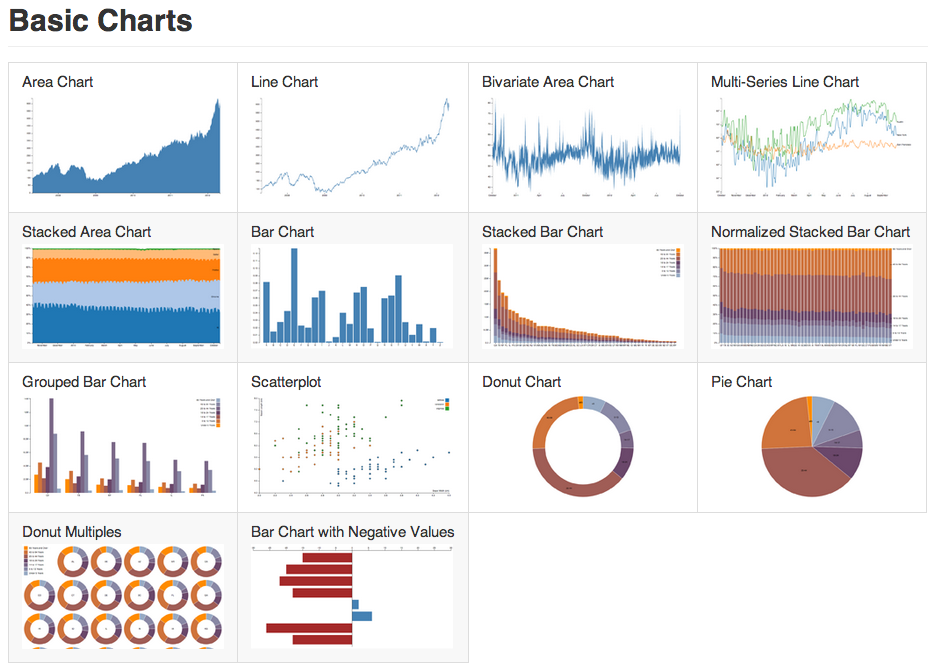
\includegraphics[width=\textwidth]{figures/d3BasicCharts.png}
  \caption[D3.js basic charts.]
    {Basic chart examples using D3.js. These are some examples of visualizations that can be tailored to visualize and interact with data cube projections in a generalized manner, building on our proposed framework.}
  \label{fig:d3basic}
\end{figure}

Several projects have focused explicitly on visualization of public data on the Web. ManyEyes was an experiment in scaling the audience for visualizations by empowering users to create visualizations of their own data \cite{viegas2007manyeyes}. ManyEyes provided a fixed set of pre-packaged visualization tools and allowed users to visualize their own data tables using the provided visualizations. GapMinder is a project aimed at exposing public data (primarily the United Nations Millenium Development Goals Indicators) using visualization \cite{rosling2005new}. GapMinder includes an animated scatter plot with an interactive time slider, a line chart showing statistics over time, and a world map (see figure \ref{fig:gapminder}). The Google Public Data Explorer provides a visual interface to selected public data sets similar to GapMinder, however it does not make the data available to users in a machine-readable format.

\begin{figure}[h!]
  \centering
  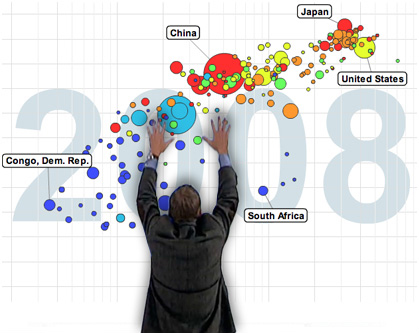
\includegraphics[width=\textwidth]{figures/gapminder.jpg}
  \caption[GapMinder and Hans Rosling.]
   {Gapminder, a public data visualization tool based on an animated scatter plot, timeline, and map. Here, Professor Hans Rosling, the creator of GapMinder, is shown gesturing the motion of the plot while presenting the visualization.}
  \label{fig:gapminder}
\end{figure}
\pagebreak
\section{Vision}
In order to motivate research in data cube integration and visualization, one must consider a larger picture. The public data available today can paint a vivid picture of the world if it is exposed in a meaningful way. Data visualization augments human cognition by enabling users to glean knowledge from data using visual perception rather than detailed mental analysis \cite{card1999readings}. Data cubes provide a well structured common representation that captures the essence of many data sets. Data visualization augments human cognition by offloading data analysis tasks to tasks of visual perception. The synthesis of public data with visualization through data cubes can lead to a technology platform that changes the world by bringing the power of data visualization to the public.

The main problem this work addresses is the gap between heterogeneous data sets and information visualization software. The reality of the current data visualization landscape contains many disparate data sets, data formats, visualization tools (specific implementations), and visualization techniques (abstract conceptual visualization approaches). The problem with this situation is that it requires an immense amount of manual work to establish a complete pipeline from any given data source to an instantiation of a visualization technique. This situation is summarized in figure \ref{fig:reality}.

\begin{figure}[h]
  \centering
  
\includegraphics[height=2in]{figures/Reality.png}
  \caption[The fragmented reality of public data visualization.]
   {The fragmented reality of public data visualization. This is the primary problem addressed by this work. }
  \label{fig:reality}
\end{figure}

An ideal solution to this problem would allow any target data set to be visualized using any target visualization technique. For example, the task ``Visualize the US Census Population Statistics on a Choropleth Map'' should be possible to execute in a straightforward way, ideally by a simple process in which the target data set is selected (US Census Population Statistics), the target visualization technique is selected (Choropleth Map), and the mapping from the data set to the visualization technique is configured (total population maps to region area color by a linear color ramp). This ideal is summarized in figure \ref{fig:ideal}.

\begin{figure}[h]
  \centering
  
\includegraphics[height=2in]{figures/Ideal.png}
  \caption[The ideal solution to the gulf between data sets and visualizations.]
   {The ideal solution to the gulf between data sets and visualizations.}
  \label{fig:ideal}
\end{figure}

Our proposed solution to address the gulf between data sets and visualization techniques involves the introduction of a generic data representation and a visualization pipeline based on it. The generic data representation should be capable of representing most public data sets. For this we chose to use the data cube concept as a foundation, as it captures the essential structure of most public data sets we considered. Additional metadata not captured by traditional OLAP systems is also required for generating satisfactory visualizations, such as provenance information and human-readable descriptions of the dimensions and measures involved. This solution is summarized in figure \ref{fig:solution}.

\begin{figure}[h]
  \centering
  
\includegraphics[height=2in]{figures/Solution.png}
  \caption[Proposed solution; generic intermediate representations.]
   {Our proposed solution; introduce generic intermediate representations conducive to data visualization.}
  \label{fig:solution}
\end{figure}

\subsection{Application Areas}
Imagine what it would be like if any person could readily access or construct interactive visualizations of public data. Public data and its visualization has relevance to many application areas including but not limited to education, journalism, and public policy.

Educational material is ripe with opportunity for augmentation by interactive visualizations. For example, consider the next generation of textbooks as eBooks running on tablets. Textbooks covering historical trends can use visualization to represent data about, for example, the distribution of various demographics across Earth and how they have shifted over the centuries. Economics courses could use interactive visualizations of global economic data to help students better understand economic dynamics. Environmental studies can include visualizations of public data on climate and pollution. Medical studies can take advantage of public health data. There is no end to the potential applications of public data visualization in education.

Journalism requires an in-depth understanding of stories as they evolve. Public data can provide context for those stories, and interactive visualizations of relevant data can be placed in digital publications alongside article text. Visualizations are already being used for this purpose today by publishers such as the New York Times and the Boston Globe.

In the area of public policy, people need to make decisions that are complex and can benefit from data analysis insights. However, public policy teams often lack the specialized skill set required to analyze available public data relevant to the decisions at hand. If tools were available that made it easy for anyone to visualize public data, policy makers could utilize such tools to great effect during the policy making process. Discussions could be augmented by explorations of public data, and policy decisions could be backed by visual data presentations that clearly and objectively make a point.

\subsection{Data}
Consider public data sources such as the United Nations, the US Census, the US Bureau of Labor Statistics, and the US Centers for Disease Control. These organizations and hundreds of others around the world are providing publicly available data about various topics including population statistics, public health, distribution of wealth, quality of life, economics, the environment, and many others. These data sets can be exposed to the general public using interactive visualization.

Most data sources provide essentially data tables. While these data tables can be mapped to visualizations, the potential for automating the visualization generation process is limited because essential metadata is missing from the table representation. For example, each column in the table may have a name, but the meaning of each column may only exist within documentation for the table, which requires manual effort to track down and integrate into the visualization. Also, with tables it is up to the visualization author to distinguish nominal (dimension) columns from quantitative (measure) columns and choose visual encodings appropriate for each. The data cube model 

The proposed data cube based data model is superior to simple data tables for several reasons. By modeling each data set as a data cube using the proposed model, the essential metadata required for automatic visualization generation is present in the data. For example, each dimension and measure of the data cube is explicit in the data representation, eliminating the need for a human to refer to external documentation as part of the visualization process. The proposed data model also explicitly represents four kinds of data relevant to visualization theory. Dimensions can be ordinal, nominal or hierarchical. Measures are quantitative. Visualization theory for ordinal, nominal and quantitative fields has been developed by Bertin \cite{bertin1983semiology}, while visualization of hierarchical data has been explored subsequently in the literature \cite{barlow2001comparison}. The explicit representation of these factors within the data model enables partial automation of visualization creation by providing visual encoding options to users based directly on visualization theory.

In addition to supporting static visualizations, our proposed data model supports interactions within and between visualizations. While tables provide minimal guidance for visualization authors in terms of possible interactions, elements of the data cube model correspond directly to visualization interactions. Measures are quantitative fields that can be used for brushing with interactive filters (for example, with rectangular selection in a scatter plot). Dimensions can be visually selected, then used for defining the slice shown in a linked visualization (for example, selecting bars in a bar chart can drive the data shown in a choropleth map). Hierarchies afford tree-based interactions such as drill-down and roll-up, which can also be used for linking visualizations. For the hierarchical dimensions of space (geographic regions) and time, pan and zoom interactions can define dimension slices.

The proposed work includes a survey of prominent public data sources. This survey will include a listing of data providers, their data access mechanisms, and data cube models of the data sets they provide. This survey of data sets will inform the development of novel data structures and algorithms capable of integrating and querying data sets from multiple sources based on the data cube model. Several data sets surveyed will be transformed into the novel data structure and integrated together as proof-of-concept examples.

\subsection{Visualizations}
There are many established data visualization techniques such as bar charts, scatter plots, and choropleth maps. Many of these techniques can be understood in terms of the data cube structure they are capable of representing. For example, a simple bar chart is capable of representing a single dimension (defining the meaning of each bar), and a single measure (defining the height of each bar). As another example, a simple scatter plot is capable of representing a single dimension (defining the meaning of each dot), and two measures (one for the X position and one for the Y position).

The proposed work includes a survey of established visualization techniques. This survey will include a listing of well known data visualization techniques and a characterization of the data cube structure they are capable of representing. For several of these visualization techniques, concrete algorithms will be developed that implement the visualization in a generic manner, building on the novel data structures and algorithms introduced for data cube integration.

\subsection{User Tasks}
End users of the system should be able to visually explore and present data for their own purposes. The data visualization process involves many steps such as importing the raw data set into the framework, identifying common dimensions and measures between data sets (schema matching), identifying when different identifiers refer to the same entity (data matching), choosing which data sets to use as input, identifying a subset (data cube projection) to use as input to a visualization, choosing which visualization technique to apply, and defining a mapping between the data cube structure and the visualization.

The proposed work includes demonstration of a complete data visualization workflow based on the data representation and visualization framework introduced. For each step in the process, it is possible to develop a user interface. However, developing a user interface for every step is beyond the scope of this dissertation. Importing data sets into the framework will require programming effort. User interface approaches will be introduced for data visualization steps that use data sets already imported into the framework, such as data set selection, querying, and visualization mapping.

\pagebreak
\section{Data Cube Representation and Integration}
The core contributions of this dissertation are novel data structures and algorithms for data cube integration and visualization. In this section these contributions are formalized. Representation and transformation of multiple data cubes lies at the heart of this project. Therefore a data structure capable of representing multiple data cubes is introduced. Algorithms are introduced for integration of multiple data cubes and for querying the integrated structure for the purpose of interactive visualization.
\subsection{Core Data Structures}
In the literature on data cubes, terminology is not always consistent. For example, Datta et al. use the term ``attribute'' to refer to dimension hierarchy levels \cite{datta1999cube}, while the RDF Data Cube Vocabulary uses the term ``attribute'' to refer to annotations on observations that may relate to scaling factors or the status of the observation \cite{rdfdatacube}. Let us begin our formalization of data cubes with a discussion of the terms that will be used: data set, dimension, level, member, cell, measure and observation.

The conceptual model of our proposed framework is shown in figure \ref{fig:udcModel}. In this figure, Crow's Foot notation \cite{hay1998making} is used to represent the concepts and their relationships. When two concepts are connected with a line that branches into three lines at one end (the ``crow's foot''), it means that there is a one-to-many relationship between those concepts. To be precise, the concept that the crow's foot points at has a cardinality constraint ``one or more'' with respect to the concept connected with the single line end. A perpendicular line to the crow's foot represents optionality (whether the relationship is mandatory or optional). When the perpendicular line is present, it means it is mandatory (not optional) that there be exactly one instance of the concept connected with the single line end present. For example, in the connection between \verb1DataSource1 and \verb1DataSet1, the crow's foot means ``A \verb1DataSet1 has many \verb1Observations1'', and the perpendicular line means ``Every \verb1Observation1 is associated with exactly one \verb1DataSet1''.

\begin{figure}[h!]
  \centering
  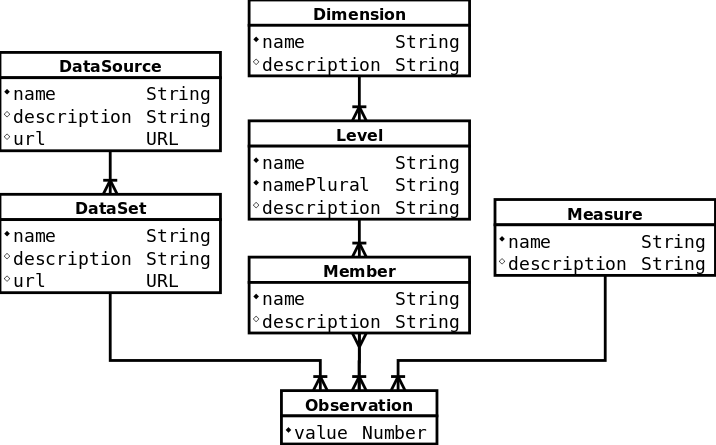
\includegraphics[width=\textwidth]{figures/UDCModel.png}
  \caption[UDC Conceptual Model.]
   {The preliminary conceptual model of our proposed unified data representation framework.}
  \label{fig:udcModel}
\end{figure}

The term ``data set'' will be used to refer to a collection of observations from the same source where each observation shares a common set of dimensions and measures. A data set can be annotated with metadata such as the title of the data set, its source, and a human readable text description. This is similar to the term \verb1DataSet1 in the RDF Data Cube Vocabulary \cite{rdfdatacube}. One example data set would be ``United Nations Population Estimates'', which contains population values at the country level since 1950.

The term ``dimension'' will be used to refer to a set of entities that may be arranged in a hierarchy. The entities within a dimension hierarchy are called ``members'' of the dimension. Members may fall into a particular ``level'', or depth of the hierarchy. One example dimension would be ``Time'', having levels ``Year'', ``Month'', and ``Day''. Members of the Time dimension at the Year level might include ``1950'', ``1951'', and so on. Space and Time are dimensions that occur in most data sets. Additional dimension examples include ``Gender'', ``Ethnicity'', ``Age range'', and ``Industry''.

The term ``cell'' will be used to refer to a set of members. Each member in a cell comes from a distinct dimension. Data sets typically include multiple dimensions. For example, the UN Population Estimates data set includes both the Space and Time dimensions. In this data set, population values are assigned to combinations of Space and Time. A specific combination of members, one from Space and one from Time, defines a cell in this data set. One example of a cell would be ``France in 1950''. The number of members defining a cell must correspond to the dimensions of the data set within which the cell is used. If the data set covers, for example, Space, Time and Gender, an example of a cell would be ``Females in France in 1950''.

The term ``measure'' will be used to refer to the properties for which numeric values can be assigned to cells. Measures almost always represent a count, sum or average over the abstract space defined by cells. For example, ``Population'' is a measure (the count of people). Other example measures include ``Average income'', ``Number of people with AIDS'', ``Child Mortality Rate'', ``Gross Domestic Product'', ``Area'', and ``Population Density''.

Some instances of these terms are universal (can be referenced by many data sets) while some are local (exist only within a data set). Dimensions, levels, members and measures are universal. Instances of these may be referenced in many data sets. Observations are local to particular data sets. This distinction of universal versus local scope is necessary when considering the challenge of integrating many data sets together, because the reconciliation of entities across independently published data sets is critical for data set integration.

Let us define universal data cube metadata as a tuple $(D, L, E, l, e, p, M)$ where
\begin{itemize}
\item $D$ is a set of dimensions.
\item $L$ is a set of levels.
\item $E$ is a set of members.
\item $l:E \rightarrow L$ is a one-to-one mapping that assigns a level to a member. Although in practice it may not make sense to assign levels to all members (for example, consider the ``Gender'' dimension), let us make the simplifying assumption that every member has a level.
\item $e:D \rightarrow E$ is a one-to-many mapping that defines the set of members that fall within a given dimension. Every member should only fall within a single dimension.
\item $p:E \rightarrow E$ is a one-to-one mapping that defines the parent-child relationship between members. For a given member $m$, $p(m)$ is its parent member in the dimension hierarchy.
\item $M$ is a set of measures.
\end{itemize}

Let us define a data set $S$ as a tuple $(D_S, L_S, E_S, M_S, C, V, g)$ where
\begin{itemize}
\item $D_S = \{d_1, d_2, \ldots , d_n \}$ is the set of $n$ dimensions present in the data set.
\item $L_S$ is the set of levels present in the data set.
\item $E_S$ is the set of members present in the data set.
\item $M_S = \{m_1, m_2, \ldots , m_k \}$ is the set of $k$ measures present in the data set.
\item $C$ is the set of cells in the data set, defined by the cartesian product of member sets for each dimension as follows: $C = e(d_1) \times e(d_2) \times \ldots \times e(d_n)$ where $e(d)$ represents the set of members in $E_S$ that fall within dimension $d$. 
\item $V$ is the set of values corresponding to observations in the data set. Each value $v \in V$ is a tuple $(u_1, u_2, \ldots , u_k)$ where each $u_i$ is a numeric value corresponding to the measure $m_i \in M_S$.
%\item $g$ is a mapping 
\end{itemize}

The proposed work involves extending this mathematical formalism of our unified data representation framework to support all operations necessary for visualization of data. More specifically, the operations introduced in the OLAP model and algebra from Datta et. al \cite{datta1999cube} including restriction (slicing), aggregation (roll-up), join, and union will be considered for extension into our model. The extension will involve handling multiple data cubes simultaneously, and dealing with the heterogeneous data cube structures that result when querying across multiple cubes.

\subsection{Integrating Multiple Data Cubes}
The data structure introduced separates the universal structural elements from the values specific to each data set. This means that when importing a data set into this data structure, a mapping between dimension and measure identifiers found in the raw data set and universal dimension and measure definitions must be established. When a data set is imported that includes dimensions or measures not found in any other data set already imported, universal dimensions and measures must be created from the data set. When a data set is imported that includes dimensions and measures shared between it and previously imported data sets, a mapping between the identifiers in the data set being imported and the existing universal definitions must be established. The process of establishing such mappings can draw from well known data integration processes of schema matching and data matching.

This approach implies that the data integration tasks of schema matching and data matching must take place before any data set is imported into the data structure. In other words, it is not possible for the data structure to contain multiple data sets for which matching has not already been done, unless duplicate universal dimensions or measures have been inadvertently created.

When querying the integrated data cube structure, heterogeneities may arise that would not occur in conventional OLAP systems. For example, two data sets may provide different values for the same measure in the same cell for dimension subsets in which they overlap. In processing query results for visualization, one approach that can be taken is to take the average of the values. This would mean that for areas in which the data sets do not overlap, values would be taken only from the single data set that provides the value, where in overlapping areas the average value from each data set will be provided. This gives the user the impression of a single uniform larger data set. The overlapping areas may also reveal discrepancies between data sets (by analyzing the differences in value), but this is an area of future research beyond the scope of this dissertation.
\subsection{Crowdsourcing Data Experiment}
Rather than manually curating data, a crowdsourcing approach can be taken to data collection for the UDC. We have performed an initial experiment to test the feasibility of this approach. Amazon Mechanical Turk supports assignment of tasks, called ``Human Intelligence Tasks'' or HITs, to workers who get paid small amounts (on the order of cents) to execute the tasks. To populate the UDC using Mechanical Turk, HITs can be devised that ask workers to find an answer to a simple question like ``What was the population of India in 1950?''. This question is an instance of a more general form ``What was the \verb1${measure}1 of \verb1${place}1 in \verb1${time}1''. By enumerating possible values for \verb1${measure}1, \verb1${place}1, and \verb1${time}1, responses to such HITs can populate large regions of the UDC.

To test the crowdsourcing data collection approach, an experiment was performed using Amazon Mechanical Turk. In this experiment, \verb1${measure}1 = population, \verb1${place}1 = \{India, China, United States\}, and \verb1${time}1 = \{1950, 2010\}. The results contained between 7 and 10 responses from multiple workers for each combination of place and time. By taking the mode (most frequently occurring value) of the worker submissions for each combination of place and time, the following table was generated:

\begin{figure}[h!]
  \centering
  \begin{tabular}{ | l | l | l | l | }
  \hline
  Place & Time & Population & Source URL \\ \hline
  India & 1950 & 369880000 & \tiny \verb1www.geohive.com/earth/population3.aspx1 \\ \hline
  China & 1950 & 563000000 & \tiny \verb1geography.about.com/od/populationgeography/a/chinapopulation.htm1 \\ \hline
  USA & 1950 & 150697361 & \tiny \verb2en.wikipedia.org/wiki/1950_United_States_Census2 \\ \hline
  India & 2010 & 1150000000 & \tiny \verb1www.indiaonlinepages.com/population/india-population.html1\\ \hline
  China & 2010 & 1339724852 & \tiny \verb1en.wikipedia.org/wiki/Demographics_of_China1\\ \hline
  USA & 2010 & 308745538 & \tiny \verb1en.wikipedia.org/wiki/United_States_Census1\\ \hline
  \end{tabular}
  \caption[MechanicalTurk Results]
   {Initial results from an experiment in crowdsourcing public data using Amazon Mechanical Turk.}
  \label{fig:crowdData}
\end{figure}

In the table shown in figure \ref{fig:crowdData}, each row represents an observation within the data cube. The values in the Place column refer to members of the Space dimension. The values in the Time column refer to members of the Time dimension. The values in the Population column assign numeric values to cells (combinations of Space and Time members) for the Population measure. This initial result demonstrates the feasibility of crowdsourced data collection for the UDC.
\pagebreak
\section{Data Cube Visualization}
The purpose of introducing novel data structures and algorithms for data cube integration is to provide a foundation for development of interactive data visualization software. Data visualization theory (the relationships between data, graphics and perception) has been explored by Bertin \cite{bertin1983semiology}, Wilkinson \cite{wilkinson2005grammar}, Mackinlay \cite{mackinlay1986automating} and others. Visualization of homogeneous data cubes has also been explored by Stolte et al. \cite{stolte2003multiscale}, Cuzzocrea et al. \cite{cuzzocrea2009olap}, and others. In the sections that follow, the possibilities for interactive visualizations based on the novel data cube integration framework are explored.
\subsection{Data Cubes and Visualization Theory}
Data cubes map well to data visualization. Bertin developed a significant part of his visualization theory based on data tables and the various kinds of fields (also referred to as attributes or columns) that one may encounter \cite{bertin1983semiology}. Dimensions and measures of data cubes, when projected into a table via querying, produce fields that correspond to the types of fields identified by Bertin. Based on an understanding of this correspondence, visualizations can be understood in terms of the data cube structures they are capable of representing.

The kinds of data table fields identified by Bertin include Nominal, Ordered, and Quantitative. Nominal fields contain references to distinct categories that have no intrinsic ordering. For example, a column in a table referring to World Countries may be considered Nominal. Ordered fields contain references to distinct categories that have an intrinsic ordering. For example a field contain the values "Small", "Medium", and "Large" may be considered Ordered. Quantitative fields contain numeric values. For example, a field containing the population of each country may be considered Quantitative. Note that any Quantitative field may be converted into an Ordered field by binning.

According to Bertin, the appropriate visual encoding of a given field in a data table is determined by whether it is Nominal, Ordered or Quantitative (from Semiology of Graphics \cite{bertin1983semiology} p. 69). The planar X and Y dimensions are the most powerful in that they are capable of representing any kind of field. Size is also capable of representing any kind of field. Value (also called luminance or brightness) is capable of precisely representing only Nominal and Ordered fields. Texture (variation in the pattern used to fill visual marks) is capable of representing Nominal or Ordered fields. Color, Orientation and Shape are only capable of representing Nominal fields.

Visualization of trees is considered in another part of Bertin's theory (as a subset of networks) and has been explored in depth in visualization literature \cite{graham2010survey} \cite{shneiderman1992tree} \cite{schulz2011treevis} \cite{barlow2001comparison}. The primary means of tree visualization include node-link diagrams, nested shapes, adjacent shapes, indented lists, and matrix representations. Node-link diagrams of trees have separate marks for each node, and each node is connected by a line. Nested shape tree visualizations such as TreeMaps or nested circles use containment to represent the tree structure. Tree visualizations using adjacent shapes such as icicle plots or tree rings (hierarchical pie charts) use adjacency to represent connections between nodes in the tree. Indented lists, as in a file system tree view or a table of contents outline, use indentation level and linear ordering to present the tree. Matrix representations from graph theory can also be used to represent trees, however this is not common.

Data cube projections produce tables whose field types derive directly from the dimensions and measures involved. Data cube dimensions may be hierarchical, ordered, or unordered. These dimensions, when projected into tables, yield trees, Ordered fields, and Nominal fields, respectively. Data cube measures always project to Quantitative fields. Using these correspondences between data cubes and data types linked with visualization methods, a taxonomy of data cube visualizations can be formulated.

Based on an understanding of how data cube projections can map to visual encodings, visualization techniques can be characterized in terms of the data cube structure they are capable of representing. The relationship between data cube structures and visual encodings provides the basis upon which generalized visualization tools can be developed. These generalized visualization tools can then be used to visualize any data cube projection that adheres to the limitations of the input data cube structure they are capable of representing. Examples of such reusable visualizations include bar chart, grouped bar chart, stacked bar chart, area plot, streamgraph, scatter plot, parallel coordinates, choropleth map, treemap, radial tree, and icicle plot.

The proposed work involves precise characterization of the above mentioned visualizations in terms of the data cube structure they are capable of representing. This categorization provides the basis upon which interactions on the visualizations can be formulated.
\subsection{Visualization Taxonomy}

\begin{figure}[h!]
  \centering
  \begin{tabular}{ | l | l | l | l | }
  \hline
  Visualization Technique & Data Cube Structure \\ \hline
  Bar Chart & 1D, 1M \\ \hline
  Pie Chart & 1D, 1M \\ \hline
  Scatter Plot & 1D, 2M \\ \hline
  Stacked Area Chart & 2D, 1M \\ \hline
  Line Chart & 2D, 1M \\ \hline
  Choropleth Map & 1D (Geo), 1M \\ \hline
  Node-Link Tree & 1D (Hierarchical), 0M \\ \hline
  TreeMap & 1D (Hierarchical), 1M \\ \hline
  Circular TreeMap & 1D (Hierarchical), 1M \\ \hline
  Icicle Plot & 1D (Hierarchical), 1M \\ \hline
  Hierarchical Pie Chart & 1D (Hierarchical), 1M \\ \hline
  Parallel Coordinates & 1D, nM \\ \hline
  Pivot Table & nD, nM \\ \hline
  Small Multiples & +1D or +2D \\ \hline
  \end{tabular}
  \caption[Visualization Taxonomy Table]
   {Our taxonomy of visualization techniques based on the data cube structures they are capable of representing. }
  \label{fig:visTax}
\end{figure}
We introduce a taxonomy of visualization techniques based on the data cube structures they are capable of representing, as shown in the table in figure \ref{fig:visTax}. In the ``Data Cube Structure'' column, ``D'' stands for Dimension and ``M'' stands for Measure. The number preceding ``D'' or ``M'' is the number of Dimensions or Measures that the visualization technique is capable of representing. When ``n'' is used instead of a number, it means an arbitrary number of Dimensions or Measures can be represented by the visualization. ``Small Multiples'' is considered here as a special case that can be applied to any existing visualization by replicating the visualization while changing the slice in 


\subsection{Prototypes}

As a first prototype, I implemented a timeline visualization of the United Nations Population Estimates data set (see figure \ref{fig:unTimeline}). To create this visualization, I manually cleaned the data originally made available as an Excel file and exported it as a CSV file. D3.js was used to create the timeline visualization from the CSV file. This example was created in order to fully understand the steps involved in visualizing a real-world public data set. This implementation has some aspects that are hard-coded to the specific data set, however this implementation can serve as a starting point for developing the generalized data representation and visualization framework incrementally.

\begin{figure}[h!]
  \centering
  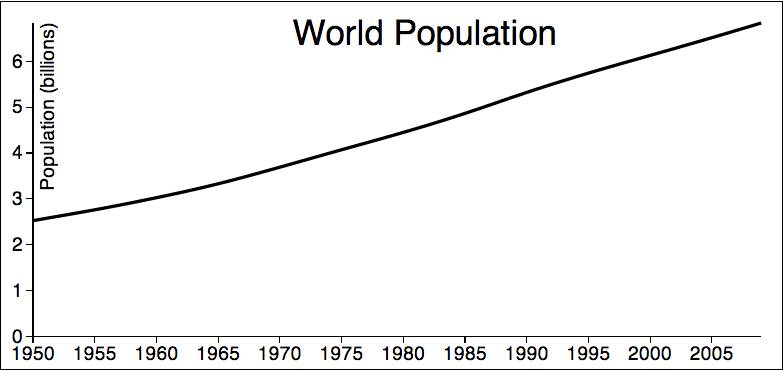
\includegraphics[width=\textwidth]{figures/unTimeline.png}
  \caption[UN Population Timeline.]
   {A timeline visualization of the United Nations Population Estimates data set. I implemented this visualization using D3.js and data downloaded from the United Nations Web site as a first prototype for visualizing public data. }
  \label{fig:unTimeline}
\end{figure}

As a second prototype, I implemented a stacked area chart of mortality data downloaded from the Centers for Disease Control, shown in figure \ref{fig:mortalityVisV2}. The data originally downloaded CSV (Comma Separated Value) file was not valid CSV, and had to be manually corrected using a text editor. The table contained a hierarchy of diseases, and all but the top-level disease categories were removed manually. Selecting the subtree of causes of death to include in the visualization is one example of a task that would be automated with our data representation framework. Next, a JavaScript program was written that pivoted the table from a format where each column was a year to a format where each row is a year, making the table usable by D3.js. This table contained an entry for ``all causes'', which was removed manually because it was not appropriate to include visualize.

The mortality data set was published using GitHub Pages using a JSON (JavaScript Object Notation \cite{crockford2006application}) structure compatible with D3.js \cite{d3}. AMD (Asynchronous Module Definition) is a JavaScript pattern for publishing and consuming reusable modules across domains \cite{osmani2012learning}. The mortality data set was published as an AMD module containing JSON data rather than as a CSV or JSON file in order to circumvent the same-origin policy. This allows any Web page to consume the data set, not only pages within the same domain. This method of publishing was chosen because it is a simple way to publish data publicly with zero cost (as GitHub Pages is a free service for Open Source code), longevity (as GitHub is less likely to go offline in the future than a private server relying on my bank account), and cross-domain availability (any page can load the module using an AMD loader such as \verb1require.js1). This method of publishing data is also developer-friendly, as most modern developers are familiar with GitHub.

The mortality stacked area visualization highlights several issues that will be faced in general when visualzing data that must be addressed by our proposed data representation framework. The causes of death extracted from the raw data are sometimes too long to use in the visualization. For example ``Symptoms, signs, and abnormal clinical and laboratory findings, not elsewhere classified'' is too long, and could be simplified to ``Unclassified conditions''. In a data cube model, causes of death would be members in a dimension hierarchy. The labeling issue encountered in the mortality visualization indicates a need to support renaming of members for use as textual elements within visualizations. Since each label refers to a dimension member which also may be a generally well-known concept, the labels on the visualization could, for example, be links to the Wikipedia pages about the various causes of death, such as Cardiovascular Disease. Also, there are 24 causes of death presented in this visualization using different colors, however D3 color scales only support up to 20 colors. This issue indicates that it may be useful to be able to automatically aggregate dimension members together as a new ``Other'' category in certain cases, or allow users to manually select only a subtree of a dimension hierarchy for visualization.

%\begin{figure}[h!]
%  \centering
%  \includegraphics[width=\textwidth]{figures/mortalityVisV1.png}
%  \caption[CDC Mortality Visualization Version 1.]
%   {A first try at a stacked area visualization of Mortality (causes of death over time) data downloaded from the US Centers for Disease Control Web site. I implemented this visualization using D3.js and manual data preprocessing.}
%  \label{fig:mortalityVisV1}
%\end{figure}

\begin{figure}[h!]
  \centering
  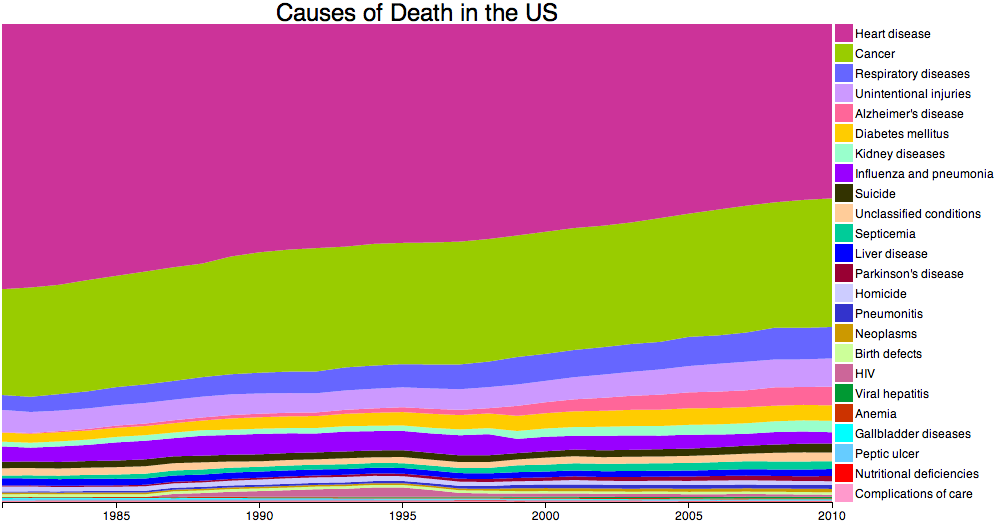
\includegraphics[width=\textwidth]{figures/mortalityVisV2.png}
  \caption[CDC Mortality Visualization Version 2.]
   {A second pass at a stacked area visualization of Mortality data from the US Centers for Disease Control. This version has 25 hand-picked distinguishable colors, a color legend to spread out labels, and shortened labels in some cases.}
  \label{fig:mortalityVisV2}
\end{figure}

Figure \ref{fig:cardiovascularDiseaseRawTree} shows a sample of the raw data from which the hierarchy of causes of death must be gleaned. In this data the hierarchy is encoded as an indented tree. Two different characters are used as indentation characters, ASCII codes 32 (space) and 65533 (unknown character). The level of indentation does not use a consistent number of indentation characters per indentation level. For example, the indentation level jumps from 0 to 4 to 7 to 10 to 13. I implemented an algorithm that parses the tree structure from an indented list and outputs the tree in a the JSON tree data structure compatible with D3.js hierarchical layouts.

Several D3 example were drawn from to implement the cause of death tree visualization shown in figure \ref{fig:mortalityVisTree}, which uses the Reingold–Tilford ``tidy'' tree layout algorithm \cite{reingold1981tidier}. This visualization shows only the hierarchy of causes of death, but no numerical values associated with each node. Notice that the two causes of death that show the highest percentages in our stacked area visualization, Cancer and Cardiovascular Diseases, are the two nodes in the hierarchy that have the two largest subtrees of categorization.

The node-link tree visualization in figure \ref{fig:mortalityVisTree} is an example of a visualization technique that can be applied to visualize dimension hierarchies in general. This implementation shows the structure of the hierarchy clearly, but has several drawbacks. Due to the size of the hierarchy, the inclusion of labels for all nodes necessitates small labels that are only legible at high resolution. When a hierarchy scales above certain thresholds of width and depth, this visualization becomes unwieldy, and labels must be truncated or omitted entirely. This is one example of scalability issues that must be addressed when developing general-purpose visualization technique implementations.

\begin{figure}[h!]
  \centering
  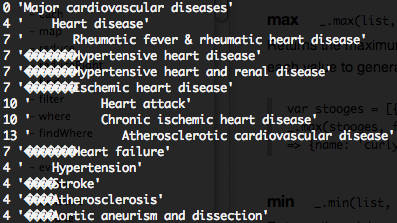
\includegraphics[width=\textwidth]{figures/cardiovascularDiseaseRawTree.png}
  \caption[Cardiovascular disease raw tree.]
   {A portion of the raw data from the Centers for Disease Control encoding the hierarchy of causes of death. The number of indentation characters is shown on the left, and the content of the ``Cause'' field from the original CSV file is shown on the right in quotes. Note that there are two different indentation characters used, and the indentation level is not of a consistent multiple. This is one example of an unconventional format that must be parsed into a dimension hierarchy for use within our data representation framework.}
  \label{fig:cardiovascularDiseaseRawTree}
\end{figure}

\begin{figure}[h!]
  \centering
  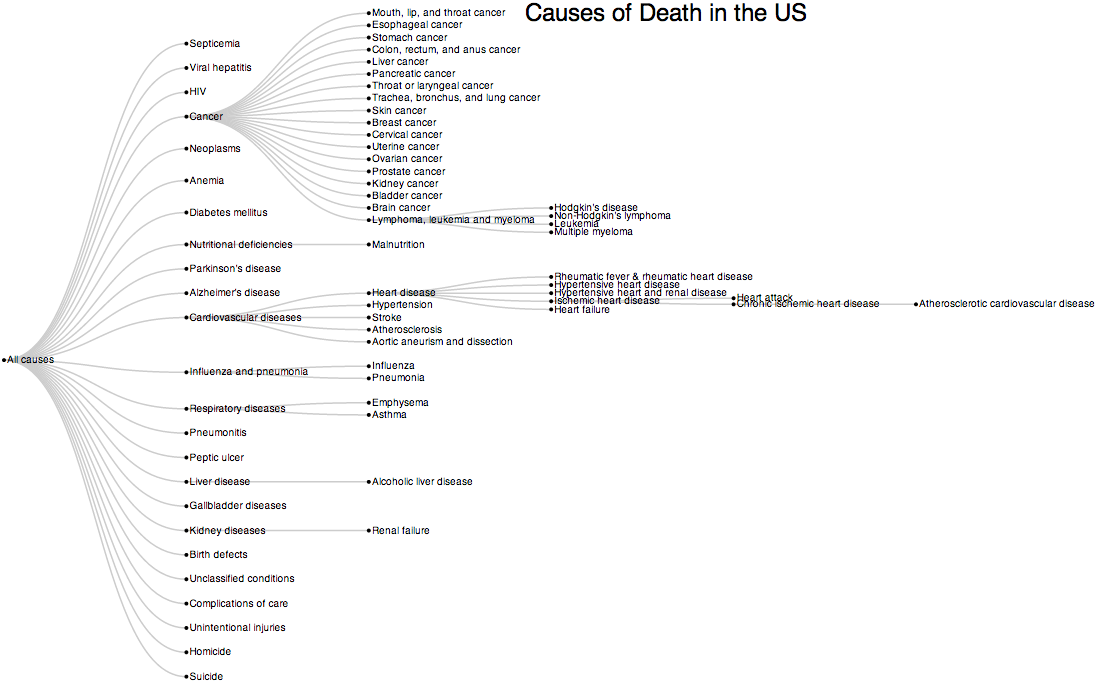
\includegraphics[width=\textwidth]{figures/mortalityVisTree.png}
  \caption[Cause of death tree visualization.]
   {A tree visualization of data from the Centers for Disease Control showing the hierarchy of causes of death. This is one example of a visualization that shows the structure of a dimension hierarchy.}
  \label{fig:mortalityVisTree}
\end{figure}

The pair of visualizations shown in figure \ref{fig:mortalityVisV4} is an example of a visualization dashboard with multiple linked views. The tree view shows a single level subtree. Black nodes have children, while white nodes do not. Clicking on a black node causes the tree to drill down into the subtree with the clicked node as its root. When this interaction is executed, the stacked area visualization is recomputed to show the new set of disease causes that correspond to the children of the newly selected tree node. In this way, the tree visualization provides interactions for drill down and roll up that define the slice of the data shown in the stacked area chart.

\begin{figure}[h!]
  \centering
  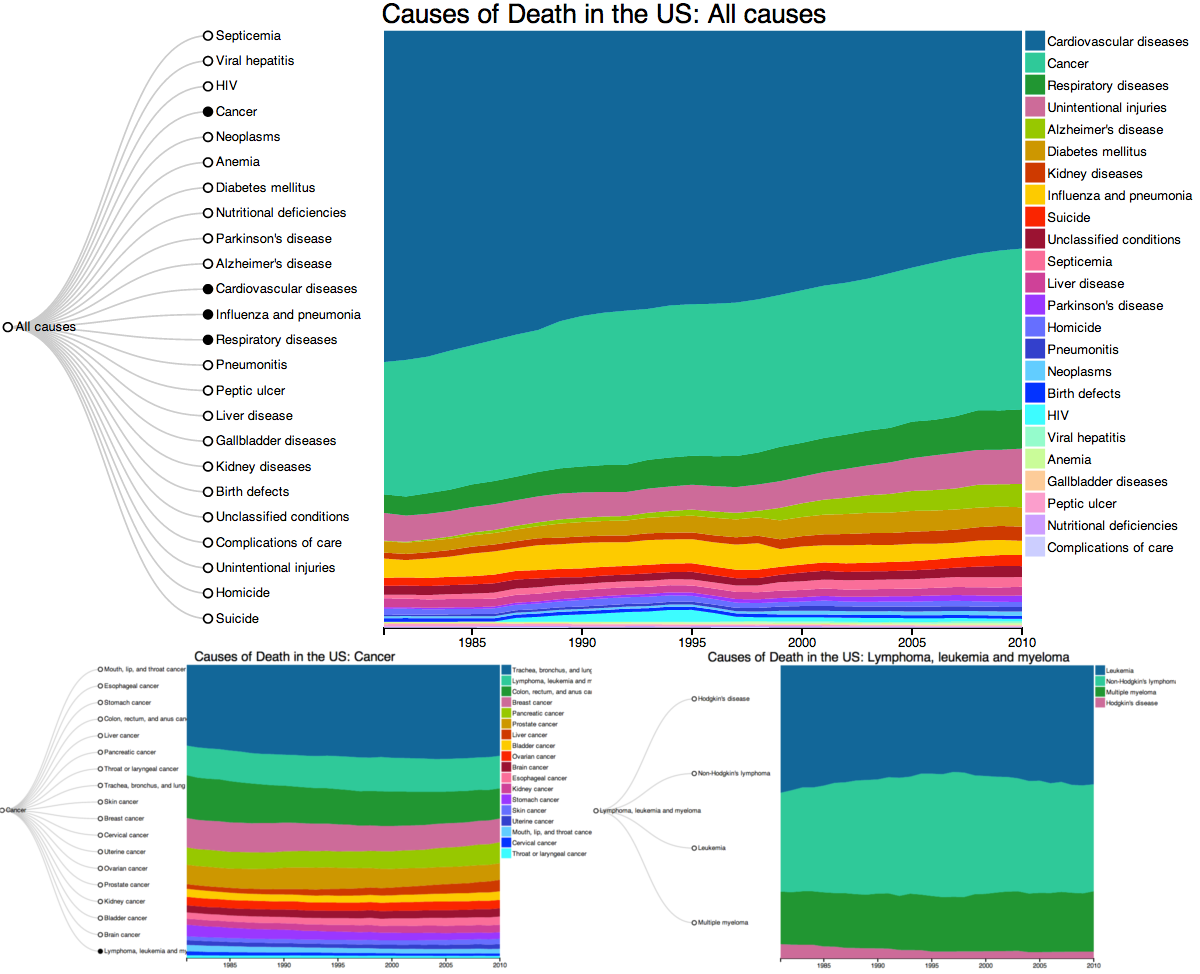
\includegraphics[width=\textwidth]{figures/mortalityVisV4.png}
  \caption[CDC Mortality Visualization with linked views.]
   {Cause of death visualization with two linked views. Navigating up and down the hierarchy by clicking on nodes changes the slice of data shown in the stacked area visualization. The top view shows the top-level causes of death. Clicking on the ``Cancer'' node yields the view on the bottom left, which shows types of cancer in the stacked area visualization. Further drilling down to ``Lymphoma, leukemia and myeloma'' yields the view on the bottom right.}
  \label{fig:mortalityVisV4}
\end{figure}

\subsection{Interactive Data Cube Visualization Dashboards}
Based on the data cube structure represented by a given visualization, interactions on the visualization can be related back to the data elements represented. For example, a rectangular selection on a scatter plot determines a subset of points. The subset of points, by inverting the visual encoding, defines a subset of the dimension members used to create the points. This subset of dimension members can be used as input to queries that define other visualizations or overlays on other visualizations. These kinds of linked interactions can be used for implementing well-known linked interactions such as brushing, linking, probing (details on demand) and interactive filtering. The proposed work includes a characterization of the interaction techniques available in each of the reusable data visualizations explored. Based on the interaction techniques available and the types of query fragments they can define, a framework for defining interactive visualization dashboards will be introduced.

Initial prototypes indicate a promising approach for representing and configuring interactive visualization dashboards. The configuration of a visualization dashboard can be represented by a tree structure corresponding to nested boxes, as well as visualization configuration options. The configuration options may contain references to elements of other visualizations on the dashboard. This is how, for example, zooming and panning on a map can be configured to interactively drive the subset of data shown in a timeline. Figure \ref{fig:dashboardConfig1} shows a simple dashboard layout configuration. Figure \ref{fig:dashboardConfig2} shows a more advanced prototype including a map component.

\begin{figure}[h!]
  \centering
  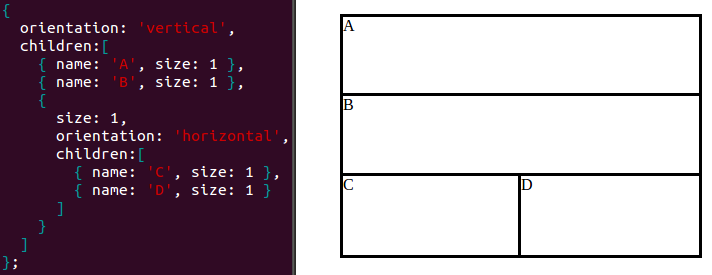
\includegraphics[height=2in]{figures/dashboardLayout.png}
  \caption[Basic dashboard layout configuration.]
   {Basic dashboard layout configuration. The nested box layout on the right is determined by the configuration definition on the left.}
  \label{fig:dashboardConfig1}
\end{figure}

\begin{figure}[h!]
  \centering
  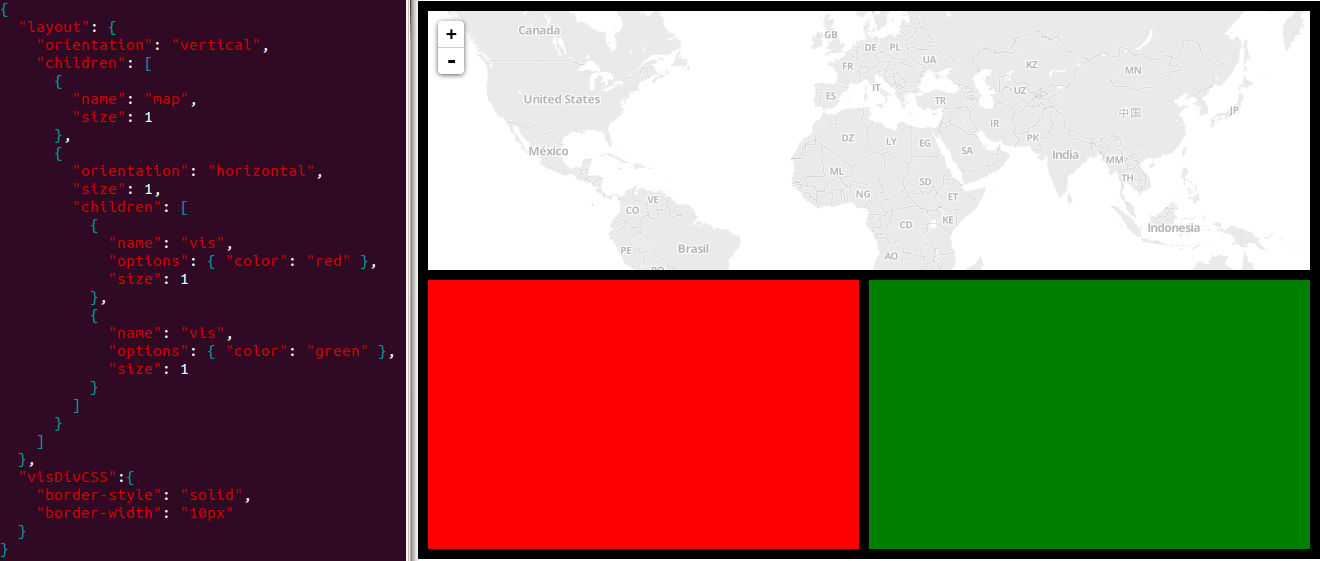
\includegraphics[height=2in]{figures/mapDash.png}
  \caption[Dashboard layout configuration and configuration of components.]
   {An example dashboard layout configuration with customized elements.}
  \label{fig:dashboardConfig2}
\end{figure}

The prototype dashboard layout system was used during a summer internship at Rapid7, a cybersecurity company, to create an interactive visualization dashboard with multiple linked views for analyzing corporate login activity (see figure \ref{fig:ingressDash}). Technologies used for visualization include D3.js, a visualization framework that uses SVG, and Leaflet.js, a framework for geographic maps. The map shows where users have logged into the network, aggregated geographically using the Leaflet MarkerCluster plugin and visualized using D3's Pie Chart layout. Black represents successful logins and blue represents failed logins. This industry application of our dashboard layout framework demonstrates its capability to define dashboards with multiple linked views. This framework has been released as Open Source and is available at \verb1github.com/curran/dashboardScaffold1.

\begin{figure}[h!]
  \centering
  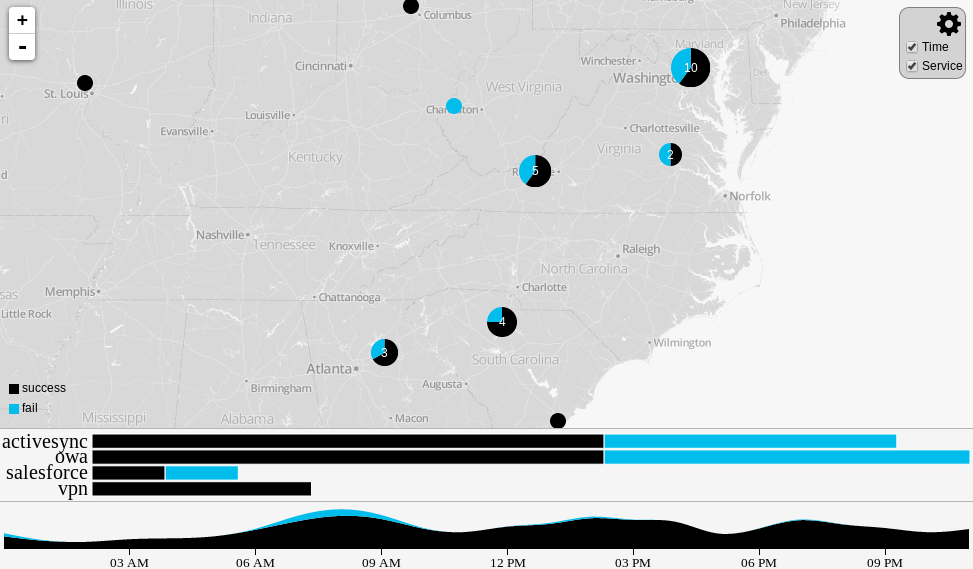
\includegraphics[width=\textwidth]{figures/mapDocs7.png}
  \caption[The Rapid7 ingress dashboard.]
   {Our open source dashboard configuration framework in use in industry. This dashboard shows corporate login data, and is integrated into the Rapid7 product called UserInsight.}
  \label{fig:ingressDash}
\end{figure}
\pagebreak
\section{Plan of Action}
In order to complete the proposed dissertation project, the following tasks will be completed:
\begin{itemize}
\item Introduce and refine a data representation framework consisting of novel algorithms and data structures capable of representing, integrating and querying multiple data cubes for the purpose of visualization.
\item Survey a substantial sample of public data sets and characterize them in terms of data access mechanisms (user interfaces, data formats and data delivery protocols) and their coverage over universal dimensions and measures.
\item Survey a substantial sample of visualization techniques and characterize them in terms of the data cube structure they are capable of representing and the interactions they afford.
\item Develop a conceptual framework for composing interactive data cube visualizations into dashboards with multiple linked views.
\item For several of the public data sets surveyed, load the data into a proof-of-concept implementation of the data representation framework that uses Web technologies.
\item For several of the visualization techniques surveyed, implement the visualization techniques in a generic manner, building on the novel data structures and algorithms introduced for data cube integration.
\item Use the generalized techniques implemented to visualize the data sets imported into the framework.
\item Generate an interactive visualization dashboard with multiple linked views that demonstrates using interactions in one visualization to define the slice of the data shown in another.
\end{itemize}
\pagebreak
\section{Expected Contributions}
In summary, the expected contributions of this dissertation include the following:
\begin{itemize}
\item Novel data structures and algorithms for data cube integration. Existing formats, protocols and models only consider the case of homogeneous data cubes computed from a single source of relational data, and do not handle the case of integrating many pre-computed data cubes from multiple sources. Data integration has been well studied for relational data, but data integration methods have not been applied to OLAP cubes, which present unique challenges including management of dimension hierarchies and measures that are ``universal'', or shared by many data sources.
\item A conceptual framework that links the integrated data cube structure with existing data visualization theory and techniques. Much work has been done concerning ``Visual OLAP'' \cite{mansmann2008visual}, however the visualization approaches for OLAP cubes have not been extended to handle the rich heterogeneous structure introduced by integrating many data cubes from multiple sources.
\item A framework for defining visualization dashboards with multiple linked views for interactively exploring integrated data cubes. Interactions between multiple views for OLAP cubes have been considered, but our proposed integrated data cube structure affords a richer set of interactions that goes beyond traditional OLAP operations such as drill-down, roll-up, slice and dice.
\end{itemize}

These contributions will advance the field of computing and data visualization by enabling the development of tools for integrating and visualizing heterogeneous data sets in ways never before possible.
\end{doublespace}
\bibliographystyle{plain}
\bibliography{proposal}
\end{document}
